%\documentclass[a4j,10pt]{ujarticle}
\RequirePackage{ifuptex,ifluatex}
\ifluatex
\documentclass{ltjsarticle}
\else
\ifupTeX
\documentclass[uplatex,dvipdfmx]{ujarticle}
\else
\documentclass[dvipdfmx]{jarticle}
\fi
\fi
%\usepackage[dviout]{graphicx}
\usepackage{graphicx}
%%%%%%%%%%%%%%%%%%%%%%%%%%%%%%%%%%%%%%%%%%%%%%%%%%%%%%%%%%%%%%%%%%%%%

\pagestyle{empty}
\sloppy\fussy
\setlength{\topmargin}{-20.4mm}
\setlength{\textheight}{271mm}
\setlength{\textwidth}{175mm}
\setlength{\oddsidemargin}{-5.4mm}
\setlength{\evensidemargin}{-5.4mm}
\setlength{\headheight}{0mm}
\setlength{\footskip}{10mm}
\renewcommand{\baselinestretch}{0.79}
\renewcommand{\textfraction}{0}\renewcommand{\floatpagefraction}{1}
\renewcommand{\topfraction}{1} \renewcommand{\bottomfraction}{1}
%%%%%%%%%%%%%%%%%%%%%%%%%%%%%%%%%%%%%%%%%%%%%%%%%%%%%%%%%%%%%%%%%%%%%
\begin{document} 
\twocolumn[
\begin{center}
{\Large TCP並列接続を用いたプログレッシブダウンロード\\における順序制御方式の実装}\\
\vspace{0.1cm}
{\large Implementation of Sequence Control Method in Progressive Download \\
	Using Parallel TCP Connections}\\
\vspace{0.2cm}
{\large 1420180  平城 光雄 Mitsuo Heijo}\\
{\large 指導教員\ \  舟阪 淳一}\\
\end{center}
]
\vspace{-5mm}
\section{はじめに}
\vspace{-2mm}
近年,効率的なコンテンツ配信を目的としたCDN等でのコンテンツの分散配置などがすでに運用されている.
このような同一のファイルが様々な場所に配置されている状況を利用して複数のサーバと同時に通信を行うことで,より高速なファイルのダウンロードを実現する方式が提案されている\cite{mhttp}\cite{proxy}.
また既存の提案ではプログレッシブダウンロードにおける動画再生等を考慮した順序制御は目的とされていない.
本研究では,性能の異なる複数のTCP接続を利用して異なるサーバから同一のファイルを分割取得する場合を想定し,リクエスト送信時に各TCP接続間の性能を比較することで到着順序逆転の発生を抑制する順序制御方式を提案する.
\vspace{-8mm}

\section{関連研究}
\vspace{-2mm}
既存研究では,複数のサーバからファイルを分割して並列ダウンロードし,順序通りにクライアントに提供する代理サーバが提案されている\cite{proxy}.
既存の提案である重複再要求方式では,非有効ブロックの個数がある閾値を超えた場合は別の接続に要求を再送信することで事後的に順序逆転に対処していた.
この提案では,要求送信時における予防的な順序逆転への対策は行われていない.
また,動画等の再生を考慮した評価も行われていない.
\vspace{-8mm}

\section{提案方式}
\vspace{-2mm}
確立したTCP接続群の中で最高性能の接続には,最若番のブロックを要求する.
最高性能の定義は使用回数が最多の接続とする.
低性能接続には前回の要求の送信からブロックの到着までのブロック送受信回数の差分\begin{math}D\end{math}を計測し,
\begin{math}D\end{math}に基づいて最若番でないブロックを要求する.
\begin{math}D\end{math}は式\ref{eq}から求める.
\begin{math}T\end{math}はその時点でのブロックの総受信回数,
\begin{math}P[X]\end{math}は接続\begin{math}X\end{math}の前回の受信完了時におけるブロックの総受信回数,
\begin{math}N\end{math}は接続の個数である.
図\ref{delay}に2つの接続間に2倍の性能差がある場合の模式図を示す.
図\ref{delay}では低性能接続の要求ブロックIDをこの性能差を考慮した要求を送信することでブロック番号0-5が順序通りの到着が期待できる様子を示している.
\vspace{-4mm}
\begin{equation}
	\label{eq}
	D = T - P[X] - N
\end{equation}
\vspace{-11mm}
\begin{figure}[h]
	\centering
	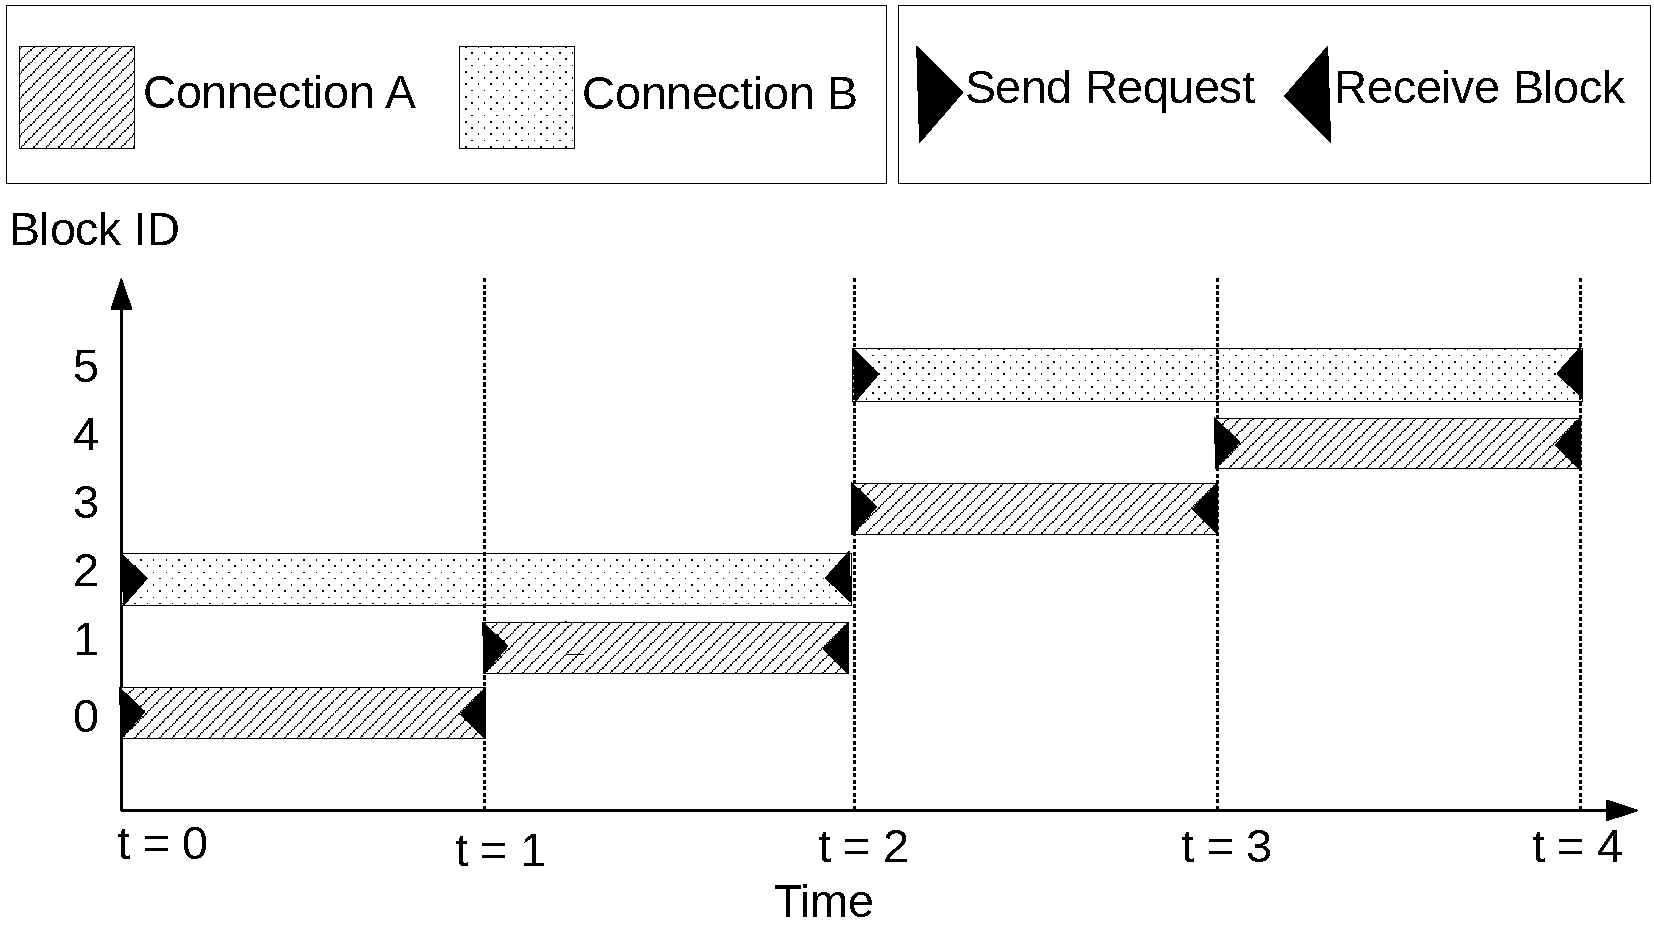
\includegraphics[width=8cm]{figure/delay.pdf}
	\vspace{-6mm}
	\caption{遅延要求の模式図}
	\label{delay}
\end{figure}
\vspace{-12mm}

\section{実験と評価}
\vspace{-2mm}
実装したプログラムでテストベッドと公開ネットワークで評価を行なった.
本稿では紙面の都合上,公開ネットワークでの結果のみを掲載する.
公開ネットワークでの実験には利用のしやすさからUbuntuのイメージファイルのパブリックミラーを使用した.
サーバは9つ使用し,2つは国内での残りの7つは国外のものを使用した.
図\ref{mirror}に事前に調査したミラーサーバにおける帯域性能の24時間変化を示す.
\ref{mirror}より国内のサーバと国外のサーバの遅延および帯域の性能差はおよそ5-10倍程度であり,15時から18時の間で帯域の変化が大きいことがわかる.
よってその時間帯に754Mbyteのファイルを各方式10回試行し,平均値を比較した.
評価対象は,先行研究で提案されている重複再要求のみを実装したもの(NORMAL)と,重複再要求に加えて提案方式である差分計測を用いた遅延要求方式を実装したもの(DIFF)の2種類である.
評価項目は,ブロックの理想到達時刻からの遅れを表す遅延時間の最大値である初期バッファリング時間,
バッファ内の非有効ブロックの数,ブロックの理想到達時刻からの正の遅れの平均である平均遅延時間である.
実験結果を表\ref{hyoka}に示す.
\vspace{-7mm}
\begin{table}[htb]
	\begin{center}
		\caption{実験結果}
		\label{hyoka}
		\vspace{-3mm}
		\scalebox{0.67}{
		\begin{tabular}{|c|c|c|c|} \hline
			方式&初期バッファリング時間[s]&非有効ブロック数&平均遅延時間[s]\\ \hline \hline
			NORMAL & 6.203 & 6.435 & 1.550 \\ \hline
			DIFF & 3.130 & 3.730 & 0.866 \\ \hline
		\end{tabular}
		}
	\end{center}
\end{table}
\vspace{-15mm}
\begin{figure}[h]
	\centering
	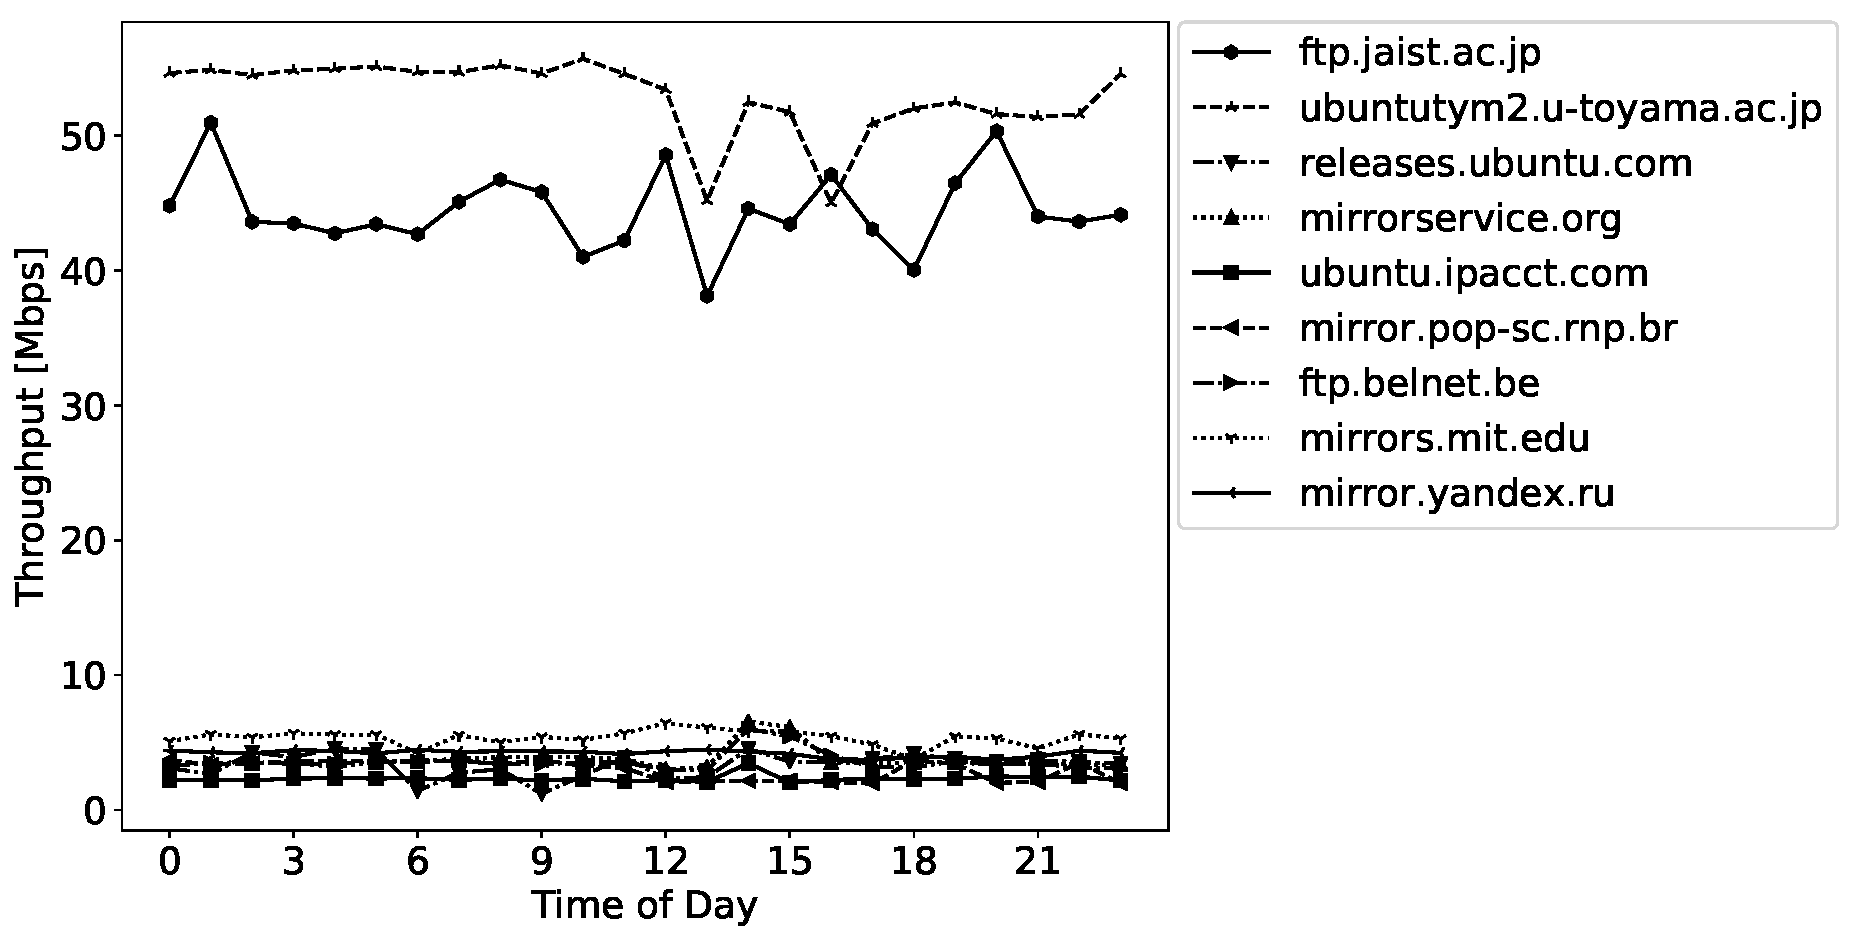
\includegraphics[width=8.5cm]{figure/thp24h-g.pdf}
	\vspace{-9mm}
	\caption{ミラーサーバにおける帯域性能の24時間変化}
	\label{mirror}
\end{figure}
\vspace{-4mm}

表\ref{hyoka}より,公開ネットワークでの評価おいて差分計測を用いた遅延予測方式は重複再要求のみの場合と比較して,
約50\%の初期バッファリング時間の短縮,約30\%の非有効ブロック数の削減,約30\%の平均遅延時間の短縮できたことが確認できる.
\vspace{-8mm}
\section{まとめ}
\vspace{-2mm}
複数のサーバから同一のファイルを並列に分割ダウンロードする際の順序逆転の発生を抑制する要求方式を提案し,
実装したHTTPクライアントをテストベッドと公開ネットワークで評価し優位性を確認した.
今後の課題としては,プロキシとして組み込んだシステムでの実際の動画の視聴体験まで含めた評価などが考えられる.
\vspace{-7mm}
%%%%%%%%%%%%%%%%%%%%%%%%%%%%%%%%%%%%%%%%%%%%%%%%%%%%%%%%%%%%%%%%%%%%%%%%%%
% 参考文献
%%%%%%%%%%%%%%%%%%%%%%%%%%%%%%%%%%%%%%%%%%%%%%%%%%%%%%%%%%%%%%%%%%%%%%%%%%
\footnotesize{
\begin{thebibliography}{2}
\vspace{-2mm}
\bibitem{mhttp}
Juhoon Kim, Yung-Chih Chen, Ramin Khalili, Don Towsley, Anja Feldmann,
"Multi-source Multipath HTTP (mHTTP): A Proposal,"
ACM SIGMETRICS Performance Evaluation Review, vol.42, no.1, pp.583--584, 2014.
\bibitem{proxy}
Junichi Funasaka, Atsushi Kawano, and Kenji Ishida: Adaptive Parallel Downloading Method for Proxy Systems, IEICE Trans., Vol.E90-B, no.4, pp.720-727, 2007.
\end{thebibliography}}

\end{document}
